\documentclass{beamer}
\usepackage[T1]{fontenc}
\usepackage[utf8]{inputenc}
\usepackage{lmodern}
\usepackage[spanish]{babel}

\mode<presentation>
{
  \usetheme{Ilmenau} 
  \usecolortheme{dolphin}
  \usefonttheme{serif} 
  \setbeamertemplate{navigation symbols}{}
  \setbeamertemplate{caption}[numbered]
} 


%%%%%%%%%%%%%%%%%%%%%%%%%%%%%%%%%%%%%%%%%%%%%%%%



\title[Plan de Investigación]{Plan de Investigación para la Tesis Doctoral}
\subtitle{\textit{Soft computing techniques applied to corporate and personal security}}
\author{Paloma de las Cuevas Delgado}
\logo{
\includegraphics[scale=0.75]{imgs/logo_ugr.png}}
\institute{Departamento de Arquitectura y Tecnología de los Computadores}
\date{\today}

\newcommand*{\vcenteredhbox}[1]{\begingroup
\setbox0=\hbox{#1}\parbox{\wd0}{\box0}\endgroup}

\newcommand{\ibmpic}{
\includegraphics[width=3cm,height=3cm,keepaspectratio]{imgs/ibm.png}}
\newcommand{\sophospic}{
\includegraphics[width=3cm,height=3cm,keepaspectratio]{imgs/sophos.png}}
\newcommand{\goodpic}{
\includegraphics[width=3cm,height=3cm,keepaspectratio]{imgs/good.png}}
\newcommand{\bphonepic}{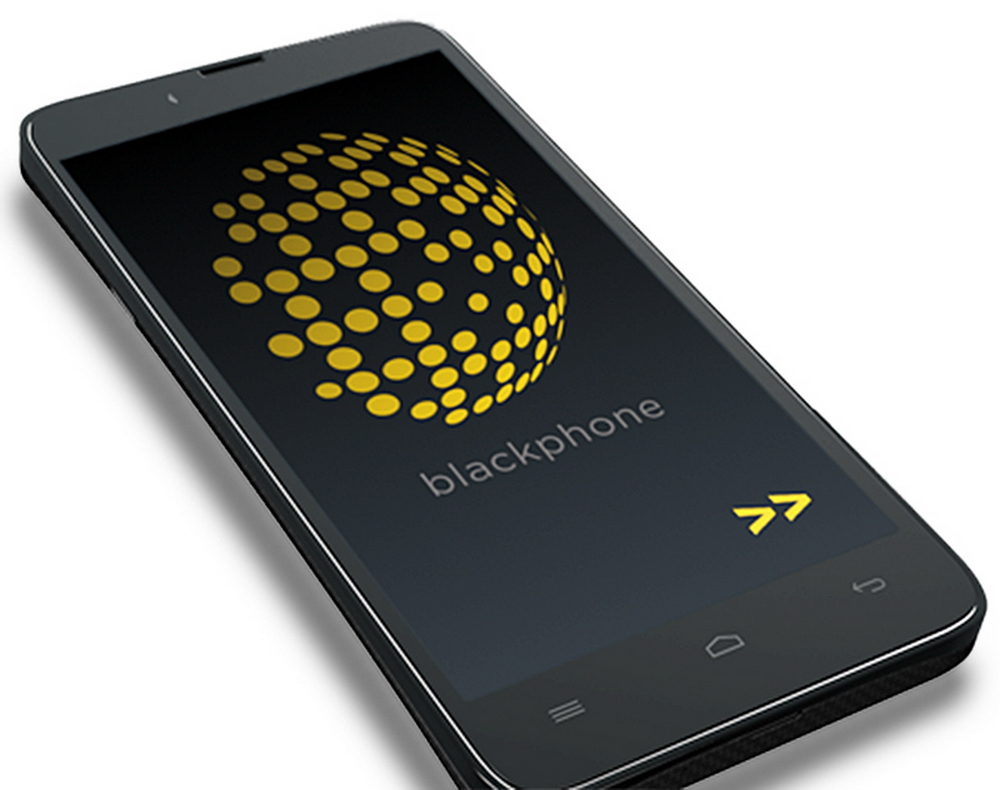
\includegraphics[width=3cm,height=3cm,keepaspectratio]{imgs/blackphone.jpg}}
\newcommand{\knoxpic}{
\includegraphics[width=3cm,height=3cm,keepaspectratio]{imgs/knox.png}}
\newcommand{\androidwpic}{
\includegraphics[width=3cm,height=3cm,keepaspectratio]{imgs/androidwork.jpg}}

\begin{document}

\begin{frame}
  \titlepage
\end{frame}

\begin{frame}{Índice}
  \tableofcontents
\end{frame}

\section{Introducción}

\begin{frame}{Introducción}

\begin{itemize}
  \item Título provisional ``Soft computing techniques applied to corporate and personal security'', o ``Aplicación de técnicas de Soft Computing a la seguridad corporativa y personal''.
\end{itemize}

\end{frame}

\section{Hipótesis}

\begin{frame}{Hipótesis}

\begin{block}{}
Big Data, Internet de las Cosas, Bring Your Own Device, La Nube, Redes Sociales
\end{block}

\begin{itemize}
  \item Términos relacionados con la inserción de dispositivos inteligentes en la vida cotidiana.
  \item Relacionados también con la posibilidad de obtener datos del \textbf{contexto} en el que se encuentran.
  \begin{block}{Contexto}
    \textit{Cualquier información que pueda usarse para caracterizar la situación de una entidad.}\footnote{{\scriptsize Abowd, G. D., Dey, A. K., Brown, P. J., Davies, N., Smith, M., \& Steggles, P. (1999). \textit{Towards a better understanding of context and context-awareness. In Handheld and ubiquitous computing} (Springer)}}
  \end{block}
\end{itemize}

\end{frame}

\begin{frame}{Hipótesis}

\begin{itemize}
  \item Las amenazas evolucionan al mismo tiempo\footnote{\scriptsize Gangula, A., Ansari, S., \& Gondhalekar, M. (2013, November). \textit{Survey on Mobile Computing Security}. In Modelling Symposium (EMS), 2013 European (pp. 536-542). IEEE.}.
  \item Sistemas de seguridad actuales: aplican unas reglas predefinidas.
  \item ¿Qué ocurre con las amenazas no conocidas?
  \item Se presenta la necesidad de que las políticas de seguridad sean autoadaptativas.
\end{itemize}

\end{frame}

\begin{frame}{Hipótesis}

\begin{block}{Hipótesis}
Demostrar que con un adecuado procesamiento de la información recopilada acerca del contexto que rodea a un usuario interaccionando con un dispositivo, además del análisis del comportamiento en el pasado, es posible adaptar el conjunto de reglas de seguridad existente y detectar de manera más precisa futuras amenazas.
\end{block}

\end{frame}

\section{Estado del arte}

\begin{frame}{Estado del arte - BYOD}

Herramientas para afrontar la introducción del BYOD:

 \vcenteredhbox{\ibmpic}
 \vcenteredhbox{\alt{\sophospic}{\phantom{\sophospic}}}
 \vcenteredhbox{\alt{\goodpic}{\phantom{\goodpic}}}
 \vcenteredhbox{\alt{\bphonepic}{\phantom{\bphonepic}}}
 \vcenteredhbox{\alt{\knoxpic}{\phantom{\knoxpic}}}
 \vcenteredhbox{\alt{\androidwpic}{\phantom{\androidwpic}}}

\end{frame}

\begin{frame}{Estado del arte - IoT}

\begin{itemize}
  \item Artículos enfocados en la parte legal de los datos que se recogen\footnote{Weber, R. H. (2010). \textit{Internet of Things–New security and privacy challenges}. Computer Law \& Security Review, 26(1), 23-30.}, \footnote{Atzori, L., Iera, A., \& Morabito, G. (2010). \textit{The internet of things: A survey}. Computer networks, 54(15), 2787-2805.}.
  \item La bibliografía se centra en securizar las comunicaciones y en la privacidad del usuario.
  \item Hay bastantes casos de uso contemplados.
  \item El trabajo de Atzori, L et al. comenta la necesidad de que en determinados casos harían falta ciertas políticas de seguridad.
\end{itemize}

\end{frame}

\section{Justificación}

\begin{frame}{Justificación}

Trabajo realizado hasta ahora:

\begin{itemize}
  \item Trabajo Fin de Máster. Estudio sobre la evolución de listas negras y blancas de URLs\footnote{Mora, A. M., De las Cuevas, P., \& Merelo, J. J. \textit{Going a Step Beyond the Black and White Lists for URL Accesses in the Enterprise by means of Categorical Classifiers}. ECTA 2014}.
  \begin{itemize}
    \item Reglas del tipo SI \textit{(url = xxxx)} ENTONCES \textit{[denegar, permitir]}
    \item Objetivo: obtener reglas que dependan de otros factores, o atributos, de la conexión HTTP.
    \item Atributos numéricos y categóricos
    \item Comparación de distintas técnicas de clasificación y de distintas configuraciones de porcentajes de entrenamiento y test.
    \item Resultados
  \end{itemize}
\end{itemize}

\end{frame}

\begin{frame}[fragile]{Justificación}

Trabajo realizado hasta ahora:

\begin{itemize}
  \item Trabajo Fin de Máster. Estudio sobre la evolución de listas negras y blancas de URLs\footnote{{\scriptsize Mora, A. M., De las Cuevas, P., \& Merelo, J. J. \textit{Going a Step Beyond the Black and White Lists for URL Accesses in the Enterprise by means of Categorical Classifiers}. ECTA 2014}}.
  \begin{itemize}
    \item Resultados
  \end{itemize}
\end{itemize}

\begin{columns}
  \begin{column}{.5\textwidth}
\begin{tiny}
\begin{verbatim}
(*)IF http_reply_code = "200"
   AND content_type = "application/json"
   AND time <= 33635000
   AND bytes <= 3921
   THEN ALLOW

(*)IF content_type = "text/plain"
   AND duration_milliseconds >= 7233.5
   THEN DENY
\end{verbatim}
\end{tiny}
  \end{column}
  \begin{column}{.5\textwidth}
\begin{tiny}
\begin{verbatim}
(*)IF content_type = "application/octet-stream"
   AND bytes <= 803
   THEN ALLOW

(*)IF bytes <= 1220
   AND time <= 33841000
   AND http_reply_code = "404"
   AND squid_hierarchy = DEFAULT_PARENT
   AND duration_milliseconds <= 233
   AND bytes <= 722
   THEN ALLOW
\end{verbatim}
\end{tiny}
  \end{column}
\end{columns}

\end{frame}

\begin{frame}{Justificación}

Trabajo realizado hasta ahora:

\begin{itemize}
  \item Escenario BYOD estudiado en el proyecto MUSES.
  \item Estudio del estado del arte en herramientas que abordan la situación BYOD.\footnote{{\scriptsize de las Cuevas, P., Mora, A. M., Merelo, J. J., Castillo, P. A., García-Sánchez, P., \& Fernández-Ares, A. (2015). \textit{Corporate security solutions for BYOD: A novel user-centric and self-adaptive system}. Revista Computer Communications (Elsevier).}}
  \begin{itemize}
    \item No existe un sistema que evolucione reglas de seguridad.
  \end{itemize}
  \item Dataset de eventos producidos por los empleados de una empresa usando MUSES para BYOD en sus dispositivos.
  \begin{itemize}
    \item Incluídos datos de contexto.
  \end{itemize}
\end{itemize}

\end{frame}


\section{Objetivos}

\begin{frame}{Objetivos}

\begin{block}{Primer objetivo}
Caracterizar una serie de entornos, o casos de uso, a contemplar para la posterior elección de métricas, técnicas, y forma de abordar los problemas.
\end{block}

Tareas del primer objetivo:

\begin{description}
  \item[1.a] Identificar los entornos que se quieren cubrir y los problemas a resolver en cada uno.
  \item[1.b] Para cada uno, identificar el contexto y datos para el análisis.
\end{description}

\end{frame}

\begin{frame}{Objetivos}

\begin{block}{Segundo objetivo}
Definir un conjunto de métricas en referencia a la detección de ataques de seguridad producidos por la insuficiencia o ineficacia de un conjunto de políticas establecido.
\end{block}

Tareas del segundo objetivo:

\begin{description}
  \item[2.a] Realizar un estudio sobre el estado del arte
    relacionado con los entornos identificados. 
  \item[2.b] Comparativa de métricas usadas en la literatura: usos, ventajas, e inconvenientes de cada una.
  \item[2.c] Definición de la métrica y justificación de la misma.
\end{description}

\end{frame}

\begin{frame}{Objetivos}

\begin{block}{Tercer objetivo}
Elegir qué técnicas de Soft Computing y de Machine Learning resultan las mejores para cada uno.
\end{block}

Tareas del tercer objetivo:

\begin{small}
\begin{description}
  \item[3.a] Estudio del arte en técnicas Soft Computing y Machine Learning aplicadas a los entornos identificados.
  \item[3.b] Relación entre la métrica escogida o definida en el segundo objetivo con las técnicas estudiadas en la tarea 3.a.
  \item[3.c] Justificación de las técnicas escogidas respecto a la métrica escogida o definida en el segundo objetivo.
\end{description}
\end{small}

\end{frame}

\begin{frame}{Objetivos}

\begin{block}{Cuarto objetivo}
Proponer una metodología que defina qué datos procesar, y cómo procesarlos, para obtener la información necesaria para adaptar las reglas de seguridad existentes.
\end{block}

Tareas del cuarto objetivo:

\begin{small}
\begin{description}
  \item[4.a] Estudio de las técnicas de pre-procesamiento y elección de una o varias, justificando el por qué.
  \item[4.b] Creación de un \textit{benchmark} para la experimentación a partir de datos reales.
\end{description}
\end{small}

\end{frame}

\begin{frame}{Objetivos}

\begin{block}{Cuarto objetivo}
Proponer una metodología que defina qué datos procesar, y cómo procesarlos, para obtener la información necesaria para adaptar las reglas de seguridad existentes.
\end{block}

Tareas del cuarto objetivo:

\begin{small}
\begin{description}
  \item[4.c] Diseñar y definir el entorno de procesamiento con las técnicas escogidas en el segundo objetivo de la tesis.
  \item[4.d] Definir cómo se validan esos resultados: comparando las métricas de cada técnica entre sí, los porcentajes de acierto en clasificación, y extrayendo conocimiento a partir de los datos.
\end{description}
\end{small}

\end{frame}

\begin{frame}{Resultado: Metodología}
La metodología estaría compuesta de varios pasos que irían detallados con las conclusiones sacadas del cumplimiento de los objetivos anteriores:

\begin{enumerate}
  \item Cómo pre-procesar los datos para un buen mantenimiento de las bases de datos y máximo rendimiento. Descripción de cómo preparar los datos antes de analizarlos.
  \item Entorno de ejecución completo, es decir, arquitectura y técnicas usadas.
  \item Validación de los resultados con técnicas propuestas, modo de uso e interpretación.
\end{enumerate}

\end{frame}

\section{Metodología de trabajo}

\begin{frame}{Metodología de trabajo}

\begin{itemize}
  \item Se propone seguir un modelo de desarrollo basado en casos de uso.
  \item Diseñar y construir un sistema que sea aplicable en sistemas reales.
  \item Primer diseño general:
\end{itemize}

\begin{center}

\includegraphics[width=0.6\textwidth]{./imgs/KRS.png}
\end{center}

\end{frame}

\begin{frame}{Minería de datos}

\begin{center}
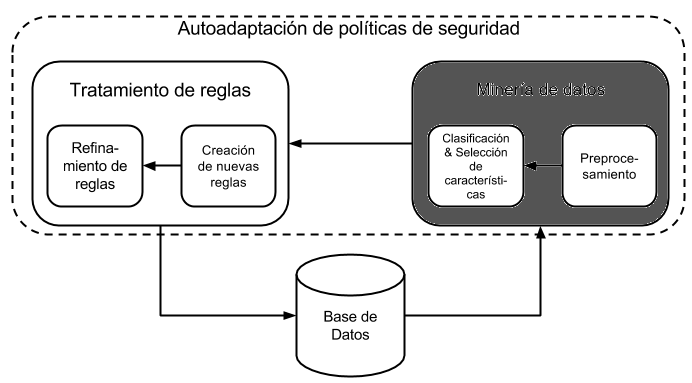
\includegraphics[width=0.4\textwidth]{./imgs/KRS1.png}
\end{center}

\begin{itemize}
  \item Tratamiento de la base de datos, eliminando ruido y corrigiendo errores.
  \item Aplicación de técnicas adicionales como selección de características.
  \item Resultado: conjunto de patrones que van al clasificador + conjunto de reglas.
\end{itemize}

\end{frame}

\begin{frame}{Tratamiento de reglas}

\begin{center}
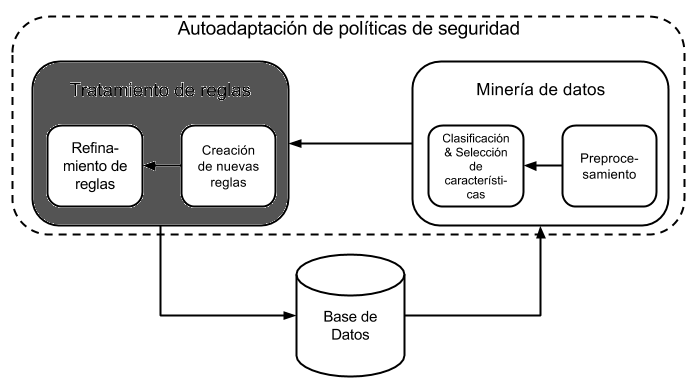
\includegraphics[width=0.4\textwidth]{./imgs/KRS2.png}
\end{center}

\begin{itemize}
  \item Comparación reglas del clasificador frente a existentes.
  \item Mantenimiento del conjunto de reglas eliminando redundancias.
  \item Aplicación de Programación genética aprovechando la estructura de árbol de una regla.
  \begin{itemize}
    \item Optimización.
    \item Mejora la comprensión de los resultados.\footnote{Tan, K. C., Tay, A., Lee, T. H., \& Heng, C. M. (2002). \textit{Mining multiple comprehensible classification rules using genetic programming}. CEC'02. IEEE.}
  \end{itemize}
\end{itemize}

\end{frame}

\section{Plan de trabajo}

\begin{frame}{Plan de trabajo}
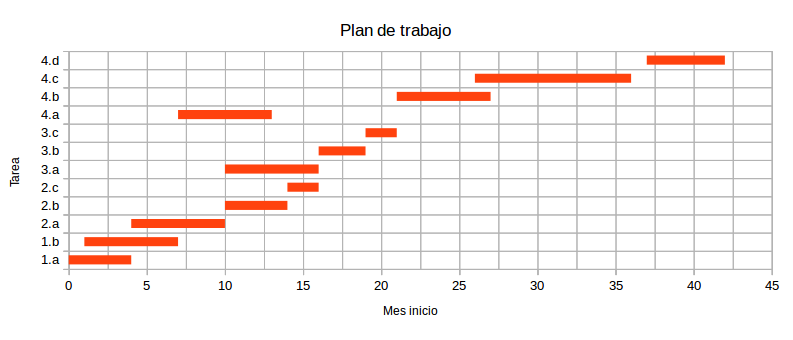
\includegraphics[width=0.95\textwidth]{./imgs/especiedegantt.png}
\end{frame}

\subsection{Medios y financiación}

\begin{frame}{Medios y financiación}

\begin{itemize}
  \item Grupo de investigación GeNeura (TIC-024) con financiación suficiente para la asistencia a congresos o para publicaciones en revista.
  \item Prevista una contratación al menos durante un año con un proyecto relacionado con la temática de la tesis.
\end{itemize}

\end{frame}

\begin{frame}
  \begin{center}
  {\large \textbf{Gracias por su atención}}
  
  palomacd@ugr.es
  \end{center}
\end{frame}

\end{document}
